\documentclass[../book.tex]{subfiles}

\chapter{Propagating subject positions}
\label{ch:subjects}

\begin{quote}
If a proposition, a sentence, a group of signs can be called
`statement,' it is not therefore because, one day, someone happened to
speak them or put them into some concrete form of writing; it is because
the position of the subject can be assigned \autocite[95]{Foucault_1972}
\index{statements!position of subject}
\end{quote}

\begin{quote}
Generalization error is what we care about \autocite{Ng_2008f}
\end{quote}

\begin{quote}
\emph{Predict if an online bid is made by a machine or a human},
`Facebook Recruiting IV: Human or Robot?' \autocite{Kaggle_2015e}
\end{quote}

Who is the subject of machine learning?
\index{machine learning!subject positions in} In early 2002, while
carrying out an ethnographic study of `extreme programming,' a software
development methodology popular at that time \autocite{Mackenzie_2004},
I spent several months visiting a company in Manchester developing
software for call centres. The software was to manage `knowledge' in
call centres such that any query from a caller could be readily answered
by staff who would query a knowledge management system to find answers
to the query. \index{knowledge!management of} This system was marketed
on the promise of machine learning. It relied on an artificial neural
network that learned to match queries and responses over time.
\index{machine learner!neural net} A taciturn neural network expert,
Vlad, sat in a different part of the room from the developers working on
the databases and the web interfaces. Vlad's work on the neural network
was at the core of the knowledge management system yet outside the orbit
of the software development team and its agile software development
processes. The rest of the team generally regarded Vlad and the neural
net as an esoteric, temperamental yet powerful component, a hidden node
we might say, of the knowledge management
system.\index{machine learner!neural net}

As we have seen with
\texttt{kittydar},\index{machine learner!\texttt{kittydar}} the position
of machine learners is changing. They are no longer exotic or
specialized, but banal or occasionally spectacular. Hilary Mason, who
was Chief Scientist at bitly.com (an online service that shortens URLs),
outlined an everyday machine learning subject position at a London
conference in 2012 called `Bacon: Things Developers Love':
\index{Mason, Hilary}

\begin{quote}
You have all of these things that are different -- engineering,
infrastructure, mathematics and computer science, curiosity and an
understanding of human behaviour -- that is something that usually falls
under the social sciences. At the intersection of all these things are
wonderful people. But we're starting to develop something new, and that
is - not that all of these things have not been done for a very long
time - but we are only just now building systems where people,
individual people, have all of these tools in one package, in one mind.
(Hilary Mason, Chief Scientist, bitly.com) \autocite{Mason_2012}
\end{quote}

These `things that are different,' what I have been calling an
operational formation, assign subject positions. In what ways does
machine learning assign subject positions? In front of an audience of
several hundred software developers, Mason describes shifts in the work
of programming associated with the growth of large amounts of data
associated with `human behaviour.' At the centre of this shift stand
`wonderful people' who combine practices and knowledges of communication
infrastructure, technology, statistics, and `human behaviour' through
curiosity and technical skills. Mason was, in effect, telling her
audience of software developers who they could become in relation to
expansive changes occurring around and in their work.
\index{programming!work!transformation of} The title of her talk was
`machine learning for hackers', and her audience were those hackers or
programmers whose coding and programming attention may have been
previously trained on web interfaces or database queries, but was now
drawn towards machine learning. A change in programming practice and a
shift towards machine learning was, she implied, the key to programmers
becoming the wonderful people, agents of their own time, capable of
doing what is only now just possible because it is all together in `one
package, one mind.'

Neural nets stand at an intersection of infrastructure and cognition,
and then propagate subject positions forwards and backwards. Their
operations encourage and eleict competitively ranking as an ordering
that not only compares human and machines, but subject positions more
generally.\index{subject positions}

\section{Propagation across human-machine
boundaries}\label{propagation-across-human-machine-boundaries}

The concatenation of `one package, one mind' does not definitively
allocate agency to people or things. (A `package' after all is another
name for a library of code.) Mason adumbrates the outline of a subject
position located at the intersection of network infrastructure,
mathematics and human behaviour.\footnote{In earlier work on machine
  learning \autocite{Mackenzie_2013}, I presented programmers as agents
  of anticipation, suggesting that the turn to machine learning amongst
  programmers could be useful in understanding how predictivity was
  being done amidst broader shift to the regime of anticipation
  described by Vincenne Adams, Michelle Murphy and Adele Clarke
  \autocite{Adams_2009}. Subsequently developments in machine learning,
  even just in the last three years, confirm that view, but in this
  chapter and in this book more generally, I focus less on
  transformations in programming practice and software development, and
  more on the asymmetries of different machine learner subjects in
  relation to infrastructures and knowledge.} Mason, herself one of
\emph{Fortune} magazines `Top 40 under 40' business leaders to watch
\autocite{CNN_2011} and also featured in \emph{Glamour}, a teenage
fashion magazine \autocite{Mason_2012}, might personify such a
`wonderful person.' \index{Mason, Hilary} She is not a lone example. In
mid-2016 Google announced a comprehensive program to re-train its
software developers as machine learners \autocite{Levy_2016}.\footnote{Other
  figures we might follow include Claudia Perlich, Andrew Ng, Geoffrey
  Hinton, Corinna Cortez, Daphne Koller, Christopher Bishop, Yann LeCun,
  or Jeff Hammerbacher. Although some women's names appear here, in any
  such list, men's names are much more likely to appear. This is no
  accident. \index{machine learner!gender of}}

`It is the privileged machine in this context that creates its
marginalized human others' writes Lucy Suchman in her account of the
encounters that `effect ``persons'' and ``machines'' as distinct
entities' \autocite[269]{Suchman_2006}.
\index{Suchman, Lucy!human-machine difference}
\index{differences!human-machine} While Mason and other relatively
well-known human machine learners are not exactly marginalized (just the
opposite, they achieve minor celebrity status in some cases), Suchman
recommends `recognition of the particularities of bodies and artifacts,
of the cultural-historical practices through which human-machine
differences are (re-)iteratively drawn, and of the possibilities for and
politics of redistribution across the human machine boundary' (285). The
intersections that machine learners currently occupy are heavily
re-distributional. In almost every instance, machine learners claim to
do something that humans alone, no matter how expert, could not. Does
the re-distribution of engineering, mathematics, curiosity,
infrastructure and `something that usually falls under the social
sciences' (but perhaps no longer does so?) both energise subjects (`its
a pretty exciting time to be in any of these things') and assign them a
marginal albeit still pivotal position in relation to privileged
machines?

Machine learner subject positions are the topic of this chapter. I focus
on artificial neural networks, or neural nets, in their various forms
ranging from the multilayer perceptron (MLP) to the convolutional neural
nets (CNN), recurrent neural nets (RNN) and deep belief networks of many
recent deep learning projects (particularly in machine learning
competitions, as discussed below \autocite{Dahl_2013}).
\index{neural net|see{machine learner!neural net}} in exploring the
re-drawing of subject-machine positions.
\index{diagram!machine learner as} Neural nets propagate between
infrastructures, engineering and human behaviour (as Mason puts it),
re-drawing human-machine differences, sometimes making it hard to seen
what subject position they entail, where subjects are located or what
they say, see and do.

Like other machine learners, neural nets re-draw human-machine
differences. Geoffrey Hinton, Simon Osindero and Yee-Why Teh
\index{Hinton, Geoffrey} writing in \emph{Neural Computation} in 2006
described a `fast learning algorithm for deep belief nets'
\autocite{Hinton_2006a}. Their description, whilst mostly couched in
terms of conditional distributions, model parameters, and error rates,
also contains a section entitled `Looking into the Mind of a Neural
Network' (1545-1546). In that section, they describe how they used their
deep belief network to \emph{generate} rather than classify
images.\footnote{In the case of this paper, and many others related to
  neural nets, the images are of hand-written digits. These digits have
  an almost constitutive role, as I discuss in this chapter.} In the
process they were able to see what the `associative memory has in mind'
(1545). The term `mind,' they comment, `is not intended to be
metaphorical' (1546) because the neural net in question has a
distributed memory of the digits it has seen. Put slightly more
formally, `the network has a full generative model, so it is easy to
look into its mind - we simply generate an image from its high-level
representations' (1529). \index{model!generative} `Looking,' as often
the case in machine learning, takes the form of diagramming a pattern,
partition or strain in the data.

The substitution of `mind' and model reproduces many aspects of the
figure of artificial intelligence (which has typically relied on
rule-based or symbolic reasoning), but the appearance of `mind' in the
form of a generative model (see chapter \ref{ch:probability}) suggests a
rather different subject position. Archaeologically, the description of
subject positions entails more than giving voice the existential threat
of artificial intelligence.\index{archaeology!subject positions}. It
first of all entails multiple positions linked to different groupings
and statements in the operational formation. As I will suggest, neural
nets are particularly interesting because they re-draw human-machine
boundaries through a combination of feeding-forward of potentials and
propagating backwards of differences specifically concerned with images.
Similarly, the practice of machine learning shifts subject positions in
a backward and forward movement. It propagates potentializing optimism
even as it undercuts the very differences that give rise to that
optimism.

\begin{verbatim}
              techniques year
\end{verbatim}

1 density estimation 2010 2 machine learning 2010 3 maximum likelihood
2010 4 heavy metals 2010 5 artificial neural networks 2010 6 crassostrea
virginica 2010

\begin{figure}
  \centering
      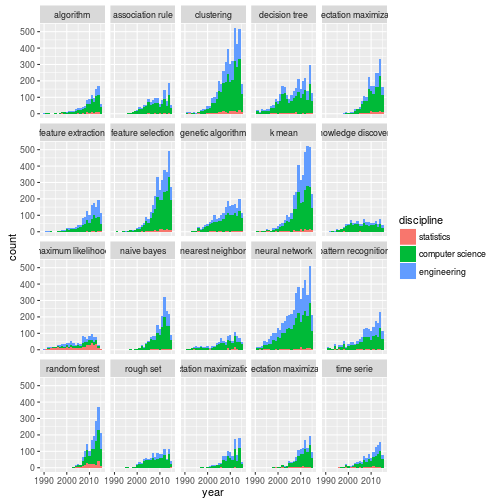
\includegraphics[width=0.9\textwidth]{figure/nn_de-1.pdf}
        \caption[Techniques and concepts most frequently mentioned]{Techniques and concepts most frequently mentioned in machine learning publication keywords, 1955-2015}
  \label{fig:disc_tech}
\end{figure}

Almost every machine learning class, textbook, demonstration, and in
recent years, machine learning competitions at some point turns to
neural nets.\index{machine learner!neural net!popularity of} Neural nets
display, however, some instability in the research literature. Figure
\ref{fig:disc_tech} shows the most frequent keywords for technical
publications across the three main disciplinary domains inhabited by
machine learners. While neural nets rank very high in computer science
and engineering disciplines (appearing just after support vector
machines), they do not appear in the statistics literature until 6 in
the rankings. The prominence of neural nets on the engineering side of
machine learning suggests a specific enunciative mapping.
\index{enunciative function!of neural net}

Neural nets are often described from a deeply split perspective. At some
moments, the description turns towards human subjects, or at least, the
brains of human subjects. At other other moments, neural nets turn
towards the vectorisation of data. \index{vectorisation} Neural nets
constantly oscillate between brain and information infrastructure. In
some ways, they renew long-standing cybernetic hopes of bring brains and
computation together in models of computational intelligence and agency
\autocite{Hayles_1999}.
\index{machine learner!neural net!cybernetics in} Although they stem
from a biological inspiration (dating at least back to the work by
McCulloch and Pitts in the 1940s
\autocites{Halpern_2015}{Wilson_2010}\index{Pitts, Walter}), they gain
traction first in the 1980s and then again from mid-2000s onwards, as
ways of dealing with changing computational infrastructures, and the
difficulties of capitalising on infrastructure that is powerful but hard
to control. In the course of fifty years, their serial re-invention --
from perceptron via neural net to deep belief net -- triply
re-distributes subject positions amidst infrastructural
re-configurations and vectorisation.
\index{infrastructure!reconfiguration of}
\index{vectorisation!of infrastructure}

For instance, writing in the 1980s, David Ackley, Geoffrey Hinton (an
important figure in the inception of neural nets over several decades),
\index{Hinton, Geoffrey!on network infrastructure} and Terrence
Sejnowski link neuroscience and semiconductors: \index{Hinton, Geoffrey}

\begin{quote}
Evidence about the architecture of the brain and the potential of the
new VLSI technology have led to a resurgence of interest in
``connectionist'' systems \ldots{} that store their long-term knowledge
as the strengths of the connections between simple neuron-like
processing elements. These networks are clearly suited to tasks like
vision that can be performed efficiently in parallel networks which have
physical connections in just the places where processes need to
communicate. \ldots{} The more difficult problem is to discover parallel
organizations that do not require so much problem-dependent information
to be built into the architecture of the network
\autocite[147-148]{Ackley_1985}.
\end{quote}

Alignments and diagrammatic overlaps between brain and `new VSLI {[}Very
Large Scale Integrated{]} technology' -- semiconductor chips --
architectures sought to reproduce the plasticity of neuronal networks in
the parallel distributed processing enabled by very densely packed
semiconductor circuits. \index{diagram!overlay} The problem here was how
to organize these connections without hardwiring domain specificity into
`the architecture of the network.' How could the architectures adapt to
the problem in hand?

We saw in chapter \ref{ch:diagram} that the psychologist Frank
Rosenblatt's perceptron \autocite{Rosenblatt_1958} first implemented
McCulloch and Pitts' cybernetic vision of neurones as models of
computation \autocite{Edwards_1996} \index{machine learner!perceptron}.
\index{Rosenblatt, Frank} While the computer science research on the
perceptron wilted under criticism from artificial intelligence experts
such as Marvin Minsky (Minsky famously showed that a perceptron cannot
learn the logical exclusive OR or \texttt{XOR} function;
\autocite{Minsky_1969}), \index{Minsky, Marvin!criticism of perceptron}
cognitive psychologists such as David Rumelhart, Geoffrey Hinton and
Ronald Williams persisted with perceptrons, seeking to generalize their
operations by connecting them together in networks (also known as
multilayer perceptrons). In the mid-1980s, they developed the
back-propagation algorithm \index{algorithm!back-propagation}
\autocites{Rumelhart_1985}{Hinton_1989}, a way of adjusting the
connections -- known as weights or parameters --
\index{parameters!weights!neural net } between nodes (neurones) in the
network in response to features in the data (see Figure
\ref{fig:rumelhart1985}).

The back-propagation algorithm directly addressed the problem of
learning to modify network organization without reliance on
problem-dependent architectures, and in without having to program them
in. \index{programmability!problem of!neural net as solution to}
Effectively, it constructs an architecture of generalization. While
cognition, and the idea that machines would be cognitive (rather than
say, mechanical, calculative, or rule-based) mesmerised research work in
artificial intelligence for several decades, the development of the
back-propagation algorithm as a way for a set of connected computational
nodes to learn came with explicit infrastructural resonances.

The resonances between computational architectures and human cognition
(centred on vision) became much more palpable from around 2006 when
`deep belief nets' appeared as a way of training many-layered neural
nets implemented on much large computational platforms
\autocite{Hinton_2006a}. These resonances continue to echo today and
indeed attract much attention.\footnote{Although mainstream media
  accounts of machine learning are not the focus of my interest here, it
  is hard to ignore the extraordinary level of interest that deep
  learning projects and techniques have attracted in the last few years.
  Articles have appeared in all the usual places -- \emph{The New York
  Times} \autocite{Markoff_2012}, \emph{Wired}\autocite{Garling_2015},
  or \emph{The Guardian} \autocite{Arthur_2015}. In many of these
  accounts, machine learning and neural nets in particular appear both
  in the guise of the existential threat of artificial intelligence and
  as a mundane device (for instance, speech recognition on a mobile
  phone). The spectacular character of deep learning could be analysed
  in terms like that of the genomes discussed in chapter
  \ref{ch:genome}. In both cases, the advent and transformation of these
  machine learners is closely linked to networked platforms (such as
  Google, Facebook, Yahoo and Microsoft) and their efforts to encompass
  within their services as many elements of experience, exchange,
  communication and power as possible. Deep learning machine learners
  currently focus mostly on images (photographs and video) and sounds
  (speech and music), and usually attempt to locate and label objects,
  words or genres.
  \index{machine learner!deep learning!existential threat of}} Like the
advent of VSLI in the early 1980s, the vast concentrations of processing
units in contemporary data centres (hundreds of thousands of cores as we
saw in the case of Google Compute in the previous chapter
\ref{ch:genome}) and in the graphics cards
\index{hardware!graphics cards} developed for high-end gaming and video
rendering (GPUs for PC gaming now typically have a thousand and
sometimes several thousand cores) pose the problem of organizing
infrastructure so that processes can communicate with each other.
Machine learners have become just as important as loose or mutable
infrastructural orders as epistemic instruments.

\begin{figure}
  \centering
      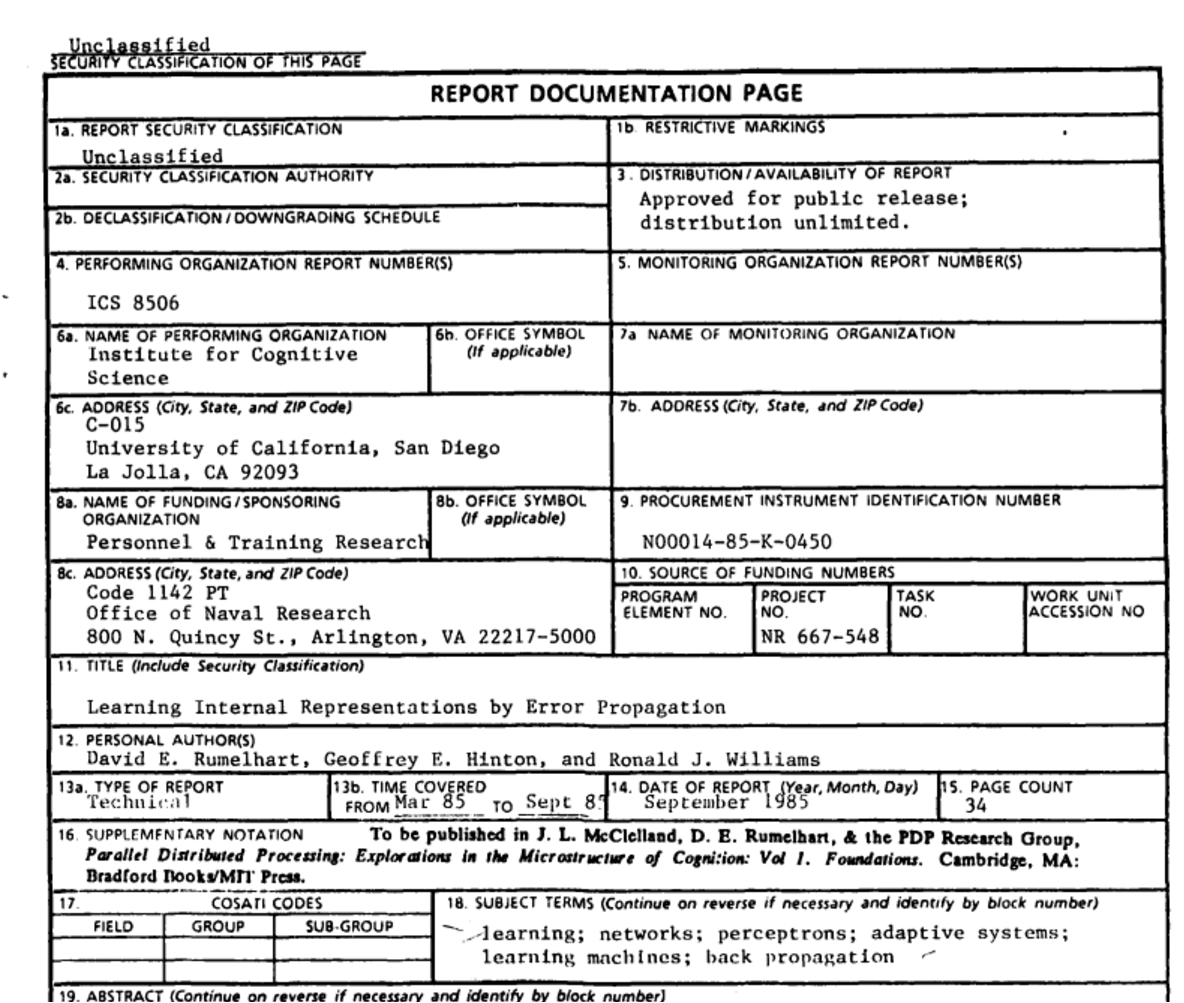
\includegraphics[width=0.9\textwidth]{figure/hinton.pdf}
        \caption[The back-propagation algorithm]{An early publication of the back-propagation algorithm (Rumelhart\_1985)}
  \label{fig:rumelhart1985}
\end{figure}

Oscillating between cognition and infrastructures, between people and
machines, neural nets suggest a way of thinking not only about how
`long-term knowledge' takes shape today, but about subject positions
associated with machine learning. \index{subject position!knowledge in}
\index{subject position!infrastructures of} As infrastructural
reorganization takes place around learning, and around the production of
statements by machine learners, both human and non-human machine
learners are assigned new positions. These positions are sometimes
hierarchical and sometimes dispersed. The machine learner subject
position is a highly relational one rather than a single concentrated
form of expertise (as we might find in a clinical oncologist,
biostatistician or geologist). Because machine learners vectorize,
optimize, probabilise, differentiate and refer, what counts as agency,
skill, action, experience and learning shifts constantly. It is
intimately bound and connected to transforms in infrastructure,
variations in referentiality (such as we have seen in the construction
of the vector space), and competing forms of accumulation or positivity.
As Suchman suggests, examining privileged machines such as neural nets
is a way to pay attention to the dispersed and somewhat disconnected
sites from which subjects program, observe, design and respond to
machine learners.

\section{Competitive positioning}\label{competitive-positioning}

How do neural nets come to oscillate between different subject
positions? The ranking of keywords in table \ref{tab:tech_disc} suggests
that machine learning as an operational knowledge formation attributes a
privileged and constitutive function to neural nets. Neural nets
concurrently spread into many difference disciplines: cognitive science,
computer science, linguistics, adaptive control engineering, psychology,
finance, operations research, etc., and particularly statistics and
computer science during the 1980-1990s. This dendritic growth did not
just popularise machine learning. It brought engineering and statistics
together more strongly. Ethem Alpaydin, a computer scientist, writes:
\index{Alpaydin, Ethem!spread of neural nets}

\begin{quote}
Perhaps the most important contribution of research on neural networks
is this synergy that bridged various disciplines, especially statistics
and engineering. It is thanks to this that the field of machine learning
is now well established \autocite[274]{Alpaydin_2010}.
\end{quote}

The forms of this field-making bridging are various.\footnote{We saw
  some use of neural nets in genomics in the previous chapter
  (\ref{ch:genome}). The initial publication of the \texttt{SRBCT}
  microarray dataset in \autocite{Khan_2001} relied on neural nets.
  \index{dataset!SRBCT}} The primary meeting point of different
disciplines has perhaps been the machine learning competitions of the
1990s that pitted neural nets against other machine learners such as
support vector machine. Many of these competitions focused on
vision-related problems such as recognising handwritten numerals. The
handwritten digits used in these competitions, particularly the Neural
Information Processing System workshops and KDD Cup (Knowledge Discovery
and Data Mining) \autocite{KDD_2013}, all come from the \texttt{mnist}
dataset and during the 1990s, much effort focused on crafting neural
nets to recognise these 60,000 or so handwritten digits.

\emph{Elements of Statistical Learning} devotes a lengthy section to the
analysis of image recognition competitions that began in the early 1990s
and continue today. Like Alpaydin, it affirms the coordinating effect of
these competitions on the development of machine learning:

\begin{quote}
This problem captured the attention of the machine learning and neural
network community for many years, and has remained a benchmark problem
in the field \autocite[404]{Hastie_2009}.
\end{quote}

As Hastie and co-authors observe, `at this point the digit recognition
datasets became test beds for every new learning procedure, and
researchers worked hard to drive down the error rates'
\autocite[408-409]{Hastie_2009}. During the 1990s, zipcodes on envelopes
(the set of handwritten digits we have already seen in chapter
\ref{ch:pattern}, the \texttt{mnist} datasets \autocite{LeCun_2012})
became a primary focus of learning. \index{dataset!\texttt{mnist}}
\index{machine learning!competitions} The many competitions focused on
the \texttt{mnist} dataset are, I suggest, a form of demonstration and
testing of machines and people that propagate machine-human differences
in machine learning. \index{data!image as}

Although they brought statistics and computer science closer, neural
networks have had a somewhat problematic position in machine learning.
Even in relation to the paradigmatic handwritten digit recognition
problem, neural nets struggled to gain purchase precisely because a
human subject position remained intimately interwoven into their
operation. On the one hand, their analogies and figurations as
sophisticated neuronal-style models suggested cognitive capacities
surpassing the more geometrical, algebraic and statistically grounded
machine learners such as linear discriminant analysis, logistic
regression, or decision trees. On the other hand, the density and
complexity of their architecture made them difficult to train. Neural
nets could easily overfit \index{overfitting} the data. As
\emph{Elements of Statistical Learning} puts it, it required `pioneering
efforts to handcraft the neural network to overcome some these
deficiencies\ldots{}, which ultimately led to the state of the art in
neural network performance'
\autocite[404]{Hastie_2009}.\index{machine learning!craft in} It is rare
to find the word `handcraft' in machine learning literature. The
operational premise of most machine learners is that machine learning
works without handcrafting, or that it automates what had previously
been programmed by hand. \index{programmining!automation of}
\index{programmability!problem of} Somewhat ironically, the competition
to automate recognition of handwritten digits, the traces that epitomise
movements of hands, entailed much handcrafting and recognition of
variations in performances of the machine.

The unstable position of subjects in relation to neural nets are
frequently discussed in contrasting terms by machine learners
themselves.\footnote{Neural nets also receive uneven attention in the
  machine learning literature. In Andrew Ng's Stanford CS229 lectures
  from 2007, they receive somewhat short shrift: around 30 minutes of
  discussion in Lecture 6, in between Naive Bayes classifiers and
  several weeks of lectures on support vector machines
  \autocite{Ng_2008b}. As he introduces a video of an autonomous vehicle
  steered by a neural net after a 20 minute training session with a
  human driver, Ng comments that `neural nets were the best for many
  years.' \index{Ng, Andrew} The lectures quickly moves on to the
  successor, support vector machines. In \emph{Elements of Statistical
  Learning}, a whole chapter appears on the topic, but prefaced by a
  discussion of the antecedent statistical method of `projection pursuit
  regression.' The inception of `projection pursuit' is dated to 1974,
  and thus precedes the 1980s work on neural nets that was to receive so
  much attention. In \emph{An Introduction to Statistical Learning with
  Applications in R}, a book whose authors include Hastie and
  Tibshirani, neural nets are not discussed and indeed not mentioned
  \autocite{James_2013}. Textbooks written by computer scientists such
  as Ethem Alpaydin's \emph{Introduction to Machine Learning} do usually
  include at least a chapter on them, sometimes under different titles
  such as `multi-layer perceptrons' \autocite{Alpaydin_2010}. Willi
  Richert and Luis Pedro Coelho's \emph{Building Machine Learning
  Systems with Python} likewise does not mention them
  \autocite{Richert_2013}. Cathy O'Neil and Rachel Schutt's \emph{Doing
  Data Science} mentions them but does not discuss them
  \autocite{Schutt_2013}, whereas both Brett Lantz's \emph{Machine
  Learning with R} \autocite{Lantz_2013} and Matthew Kirk's
  \emph{Thoughtful Machine Learning} \autocite{Kirk_2014} devote
  chapters to them. In the broader cannon of machine learning texts, the
  computer scientist Christopher Bishop's heavily cited books on pattern
  recognition dwell extensively on neural nets
  \autocites{Bishop_1995}{Bishop_2006}. Amongst statisticians, Brian
  Ripley's \emph{Pattern Recognition and Neural Networks}
  \autocite{Ripley_1996}, also highly cited, placed a great deal of
  emphasis on them.\index{Ripley, Brian} But these textbooks stand out
  against a pointillistic background of hundreds of thousands of
  scientific publications mentioning or making use of neural nets since
  the late 1980s in the usual litany of fields -- atmospheric sciences,
  biosensors, botany, power systems, water resource management, internal
  medicine, etc. This swollen publication tide attests to some kind of
  formation or configuration of knowledge invested in these particular
  techniques, perhaps more so than other I have discussed so far (
  logistic regression, support vector machine, decision trees, random
  forests, linear discriminant analysis, etc.).} They often point to a
transformation in the work of machine learning:

\begin{quote}
Neural networks went out of fashion for a while in the 90s - 2005
because they are hard to train and other techniques like SVMs beat them
on some problems. Now people have figured out better methods for
training deep neural networks, requiring far fewer problem-specific
tweaks. You can use the same pretraining whether you want a neural
network to identify whose handwriting it is or if you want to decipher
the handwriting, and the same pretraining methods work on very different
problems. Neural networks are back in fashion and have been
outperforming other methods, and not just in contests
\autocite{Zare_2012}.
\end{quote}

The somewhat vacillating presence of neural nets in the machine learning
literature itself finds parallels in the movements of individual machine
learners. Yann Le Cun's work on optical character recognition during
1980-1990s is said to have discovered the back-propagation algorithm at
the same time as Rumelhart, Hinton and Williams
\autocite{Rumelhart_1986}. His implementations in \texttt{LeNet} won
many research machine learning competitions during the 1990s. In 2007,
Andrew Ng could casually observe that neural nets \emph{were} the best,
but in 2014, Le Cun find himself working on machine learning at Facebook
\autocite{Gomes_2014}. \index{Le Cun, Yann} Similarly, the cognitive
psychologist Geoffrey Hinton's involvement in the early 1980s work on
connectionist learning procedures in neural nets and subsequently on
`deep learning nets' \autocite{Hinton_2006} delivers him to Google in
2013. \index{Hinton, Geoffrey}

Trajectories between academic research and industry are not unusual for
machine learners.\index{subject position!sites} Many of the techniques
in machine learning have been incorporated into companies later acquired
by other larger companies. Even if there is no spin-off company to be
acquired, machine learners themselves have been assigned key positions
in many industry settings. Corinna Cortes, co-inventor with Vladimir
Vapnik of the support vector machine, heads research at Google New York
\index{Cortes, Corinna}. In 2011, Ng led a neural net-based project at
Google that had, among other things, detected cats in millions of hours
of Youtube videos.\footnote{Unlike the cats detected by
  \texttt{kittydar,} the software discussed in the introduction to this
  book, the Google experiment did not use supervised learning. The deep
  learning approach was unsupervised \autocite{Markoff_2012}. That is,
  the neural nets were not trained using labelled images of cats.} Ng
himself in 2014 began work as chief scientist for the Chinese search
engine, Baidu leading a team of AI researchers specializing in `deep
learning,' the contemporary incarnation of neural nets
\autocite{Hof_2014}
\index{deep learning|see{machine learner!deep learning}}.
\index{Ng, Andrew} \index{sites!Baidu} In recent years, (2012-2015),
work on neural nets has again intensified, most prominently in
association with social media platforms, but also in the increasingly
common speech and face recognition systems found in everyday services
and devices. Many of these neural nets are like \texttt{kittydar}
\index{machine learner!\texttt{kittydar}}, but implemented on a much
larger and more distributed scale (for instance, in classifying videos
on Youtube). In contemporary machine learning competitions, as we will
see, neural nets again surface as intersectional machines,
re-distributing differences between humans and machines.

\section{A privileged machine and its diagrammatic
forms}\label{a-privileged-machine-and-its-diagrammatic-forms}

What accounts for the somewhat uneven fortunes of the neural net amongst
machine learners? The unevenness of their performance, from limited
curiosity in the late 1960s to handcrafted best-in-class performer in
the machine learning image classification competitions of the 1990s,
from second best competitor in late 1990s to the spectacular promise of
deep belief networks amidst the `awesome materiality' of social media
image streams in 2012, suggests that some powerful dynamics or becomings
are in play around them. These dynamics are not easily understood in
terms of celebrity machine learners (human and non-human) suddenly
rising to prominent or privileged positions in the research departments
of social media platforms.\footnote{In any case, social media and search
  engines cannot be understood apart from the machine learning
  techniques that have been thoroughly woven through them since their
  inception. Hence \emph{Elements of Statistical Learning} devotes
  several pages to Google's famous \emph{PageRank} algorithm, describing
  it as an unsupervised learner \autocite[576-578]{Hastie_2009}.
  \index{social media platforms!machine learning as part of}} Nor does
it make sense to attribute the rising fortunes of the neural net to the
algorithms themselves, as if some decisive advance occurred in
algorithms.

The algorithms such as back-propagation used in neural nets have not, as
we will see, been radically transformed in their core operations since
the 1980s, and even then, the algorithms themselves (principally
gradient descent \index{gradient descent}) were not new. There have been
important changes in scale (similar to those described in the previous
chapter in the case of the \texttt{RF-ACE} algorithm and Google
Compute), but as is often the case in machine learning, their
proliferation occurs through re-distributions of knowledge and
infrastructure associated with altered subject positions. While machine
learners in their machine form can be assigned a privileged position in
the transformations of knowledge and action, human machine learners are
not exactly marginalized, at least in celebrated cases such as Ng, Le
Cun, Hinton and others. Rather, we can see varying subject positions
emerging in relation to specific devices and data forms (images, sounds,
documents) in specific sites (social media platforms and mobiles devices
in particular).

A varying subject position surfaces in the operational architecture of
neural nets. Despite differences in diagrammatic form, neural net share
much with other machine learners. The language of brain, neurones and
cognition associated with neural net covers over their much more
familiar vector space and function-finding optimisations they rely on.
Diagrammatic groupings and lines of movement operate in neural nets to
expand their architecture in alignment with a series of well-established
transformations. `The central idea,' write Hastie and co-authors, `is to
extract linear combinations of the inputs as derived features, and then
model the target as a nonlinear function of these features. The result
is a powerful learning method, with widespread applications in many
fields' \autocite[389]{Hastie_2009}. The `central idea' can be seen in
the algebraic expressions that Hastie and co-authors provide for the
basic neural net model:

\begin {equation}
\label {eq:nn}
\begin {split}
Z_m = \sigma(\alpha_0m + \alpha_m^TX) m = 1, ...,M\\
T_k = \beta_0k + \beta_k^TZ, k = 1, ..., K,\\
f_k (X) = g_k (T), k = 1, ..., K,
\end {split}
\end {equation}

\begin{quote}
where \(Z = (Z_1 , Z_2, ..., Z_M )\), and
\(T = (T_1 , T_2 ,..., T_K )\). The activation function \(\sigma(v)\) is
usually chosen to be the sigmoid \(\sigma(v) = 1/(1 + e - v )\)
\end{quote}

\begin{quote}
\autocite[392]{Hastie_2009}
\end{quote}

Equation \ref{eq:nn} diagrams some familiar elements as well as some
novelty. Some elements of the neural net are already familiar from
linear models. The neural networks transform data in a vector space
denoted by \(X\). That is common to nearly all machine learners. They
make use of the non-linear sigmoid function \index{function!sigmoid}
that lies at the heart of one of the main linear classifiers used in
machine learning, logistic
regression.\index{machine learner!logistic regression} Their training
and learning processes have come to rely on the same kinds of cost, loss
or error functions \index{function!cost} we have seen in other machine
learners. \index{machine learner!neural net!central idea of}

The apparently increasing power of neural nets to learn (to see, to
find, to classify, to rank, to predict) owes much to diagrammatic
substitutions that recombine operations of past machine learners in new
intersections. These movements appear in the
equations.\index{diagrammatic!substitution} Equation \ref{eq:nn} has
three lines rather than one, and this layering and its diagonal patterns
of indexical referencing running between subscripts distinguishes neural
nets from the linear models it assembles. \index{diagram!equation as}

\begin {equation}
\label {eq:linear_model_2}
\hat{Y} = \hat{\beta_0}  + \sum^p_{j=1} X_j \hat{\beta_j}
\end {equation}

Whereas the standard linear model \index{linear model} shown in Equation
\ref{eq:linear_model_2} indexes a single vector space \(X_j\) and
approximates it using a single function \(\hat{Y}\) by searching for the
values of the parameters \(\beta_j\) that best incline a flat plane
through the data, the three lines shown in equation \ref{eq:nn} are
woven through each other much more consecutively. Each lines derives
`features' from the line above, adding layers to the network. So-called
`hidden layers,' such as line two of equation \ref{eq:nn} repeatedly
transform the vector space inside the model itself. Each node, \(1..K\),
adds a new dimension to this internal vector space. In many layered deep
learning neural nets, the dimensionality of the vector space vastly
expands. \index{vector space} Much hinges on the unobstrusive sigmoid
function operator written as \(\sigma\): `a neural network can be
thought of as a nonlinear generalization of the linear model, both for
regression and classification. By introducing the nonlinear
transformation \(\sigma\), it greatly enlarges the class of linear
models' \autocite[394]{Hastie_2009}. \(\sigma\), it seems, allows neural
nets to generalize beyond the linear model.\footnote{Recent work on deep
  belief networks replaces the sigmoid function with other non-linear
  functions that subtly alter the way layers of neural nets relate to
  each other. See \autocite{Glorot_2010} for an account of changing
  training practices in neural nets.}

\section{Varying subject positions in
code}\label{varying-subject-positions-in-code}

The operational diagram of neural nets, I would suggest, ascribes
subject positions associated with it. How does that happen? Some
familiar diagrammatic operations immediately appear in almost any actual
example of a neural net. In the code vignette shown below, the dataset
is a spreadsheet of information about passengers of the Titanic. The
\texttt{titanic} dataset, like \texttt{iris} or \texttt{boston} is often
used in contemporary machine learning pedagogy.
\index{dataset!\texttt{titanic}} It is for instance, the main training
dataset used by (kaggle.com){[}http://kaggle.com{]}, an online machine
learning competition site I will discuss below \index{Kaggle.com}. The
first few lines of the \texttt{R} code load the dataset and transform it
into vector space. For instance, variables such as \texttt{sex} that
take values such as \texttt{male} and \texttt{female} become vectors of
\texttt{1} and \texttt{0} in a new variable \texttt{sexmale}.

\begin{lstlisting}[language=R, caption={Neural net for \texttt{titanic} dataset}, label={lst:titanic_nn}]

```r
library(neuralnet)
titanic = read.csv("data/titanic3.csv", stringsAsFactors = FALSE)
titanic_transformed = as.data.frame(model.matrix(~survived + age + pclass + 
    fare + sibsp + sex + parch + embarked, titanic))
train_index = sample.int(nrow(titanic)/2)
titanic_train = titanic_transformed[train_index, ]
titanic_net = neuralnet(survived ~ age + pclass + fare + sexmale + sibsp + parch + 
    embarkedC + embarkedQ + embarkedS, data = titanic_train, err.fct = "ce", 
    linear.output = FALSE, rep = 1, hidden = 3, stepmax = 1e+05)
titanic_test = titanic_transformed[-train_index, ]
test_error = round(sum(0.5 < compute(titanic_net, titanic_test[, -c(1, 2)])$net.result)/sum(titanic_test$survived), 
    2)
```

```
## Error in nrow[w] * ncol[w]: non-numeric argument to binary operator
```
\end{lstlisting}

The line of the code that constructs a neural net using the
\texttt{neuralnet} library \autocite{Fritsch_2012} closely resembles the
lines of code used to construct linear models for the \texttt{prostate}
data (see chapter \ref{ch:vector}). The \texttt{R} formula for the
neural net looks very similar to other machine learners such as logistic
regression. It models whether someone \texttt{survived} the wreck of the
Titanic in terms of their age, class of fare (\texttt{pclass}), sex,
number of siblings/spouse (\texttt{sibsp}), number of parents/children
(\texttt{parch}) and port of departure:

\texttt{survived\ \textasciitilde{}\ age\ +pclass\ +\ fare\ +\ sexmale\ +\ sibsp\ +\ parch\ +\ embarkedC\ +\ embarkedQ\ +\ embarkedS}

\texttt{R} model formula express the response or target variable
\texttt{survived} as a combination of other variables. In this case, the
plus sign \texttt{+} indicates that the combination is linear or
additive. If this model formula looks so similar to other machine
learning techniques we have been discussing, what do neural networks
add? Why did and do so many machine learners turn to them?

Perhaps the only distinctive feature of the code listing
\ref{lst:titanic_nn} appears in the expression \texttt{hidden\ =\ 3.}
This architectural feature does not appear in the model formula in the
\texttt{R} code but does, as we have already seen, operate in the lines
of equation \ref{eq:nn}. These `hidden units' are key to neural net
since they construct the `derived features' that the model learns from
the input data \(X\).

How many nodes are hidden and in what topology matters less than the
existence of operation that allows their topology to be configured in an
encounter with data. The novelty of this operation was central to
research into neural nets. As Rumelhart, Winton and Williams announce
the algorithm in a letter to \emph{Nature} in 1986 entitled `Learning
representations by back-propagating errors'
\index{algorithm!back-propagation}:

\begin{quote}
We describe a new learning procedure, back-propagation, for networks of
neurone-like units. The procedure repeatedly adjusts the weights of the
connections in the network so as to minimize a measure of the difference
between the actual output vector of the net and the desired output
vector. As a result of the weight adjustments, internal `hidden' units
which are not part of the input or output come to represent important
features of the task domain, and the regularities in the task are
captured by the interactions of these units. The ability to create
useful new features distinguishes back-propagation from earlier, simpler
methods such as the perceptron-convergence procedure
\autocite[533]{Rumelhart_1986}. \index{error!back-propagation of}
\end{quote}

Again, despite the persistent reference to biology, the description of
the `new learning procedure' sound more like machine learning. There is
talk of minimizing a measure of difference between actual and desire
output vectors (optimizing through a cost or loss function), as well as
mention of `features' and `weights' (usually a synonym for model
parameters: `the neural network model has unknown parameters, often
called weights, and we seek values for them that make the model fit the
training data well' \autocite[395]{Hastie_2009}). The novelty, however,
consists in the `hidden' units whose interactions `represent important
features.' In other words, the flat additive combination of features
expressed in the \texttt{R} model formula above does not convey the
interactions of these units. (As Hastie and co-authors put it, `the
units in the middle of the network, computing the derived features
\(Z_m\), are called hidden units because the values \(Z_m\) are not
directly observed' \autocite[393]{Hastie_2009}.) These units can only
viably interact in the neural nets because the back-propagation
algorithm offers a way to create `useful, new features' from the data.
But because they interact through back-propagation, the hidden units
`capture' regularities in the `task domain' and thereby do what counts
as cognition in the connectionist philosophies associated with neural
nets (see the PDP group's work \autocite{McClelland_1986}).

The hidden layers lend a network form to machine learning. The final
diagrammatic form in which neural nets appear is the network. Network
graphs already appeared in Rosenblatt's perceptron work
\autocite{Rosenblatt_1958}, but they ramify tremendously in the
aftermath of back-propagation. Almost every book and article relating to
neural net presents some version of the diagram shown in Figure
\ref{fig:titanic_net}.

\begin{verbatim}
## Error in plot.nn(titanic_net, fontsize = 8, show.weights = FALSE): weights were not calculated
\end{verbatim}

\begin{figure}
  \centering
      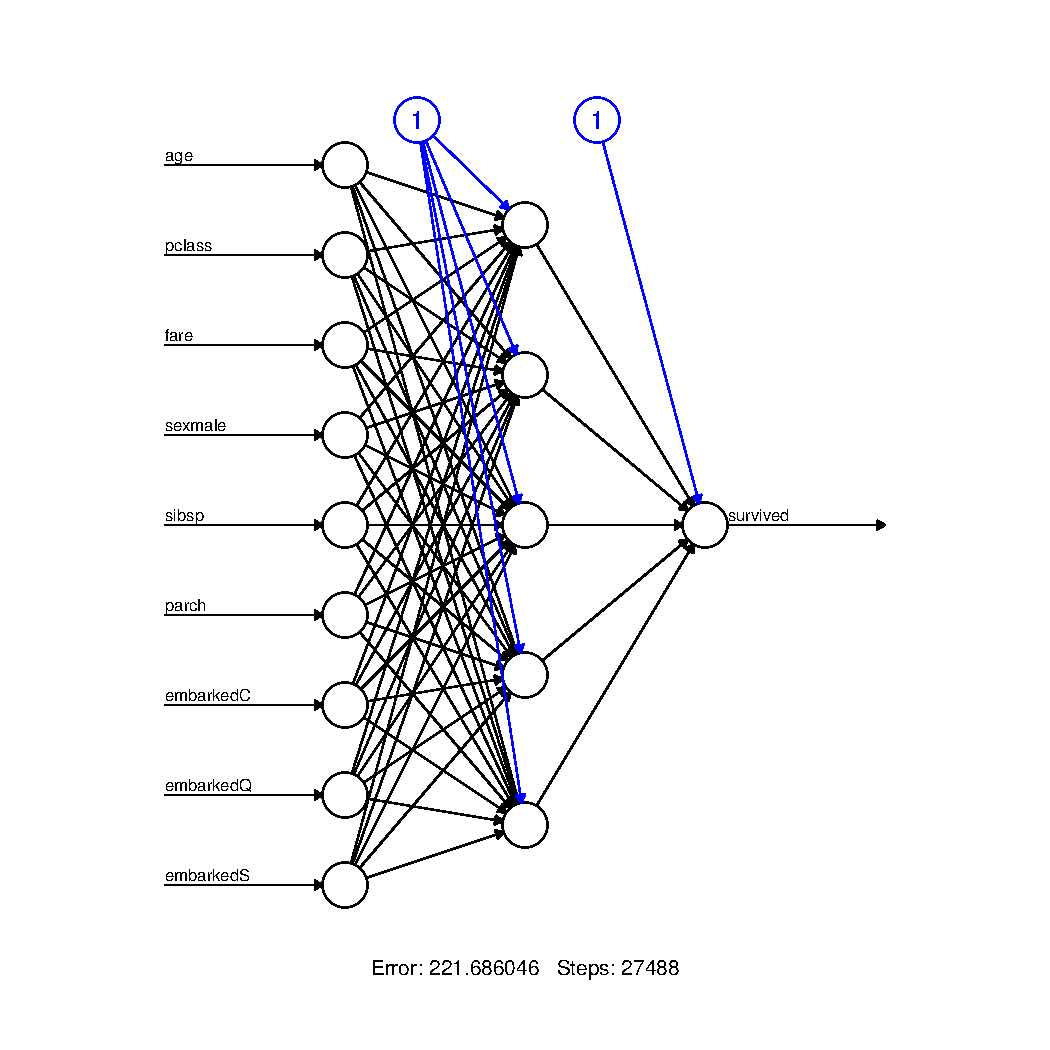
\includegraphics[width=0.9\textwidth]{figure/titanic_net.pdf}
        \caption{Neural network topology for 3-hidden unit `titanic` data}
  \label{fig:titanic_net}
\end{figure}

Although the network topology of the model appears in many more
complicated forms, it diagrams several operations. First, it presents a
surface -- the input layer -- that indexes something in the world.
\index{diagram!network} \index{graphic!network} The input layer, shown
as \(X\) in the algebraic diagram of equation \ref{eq:nn}, suggests
receptive or recording surface (for instance, a camera). Early neural
net papers on the handwritten digital recognition problem sometimes
describe cameras mounted above tables focused on images
\autocite{LeCun_1989}. Second, it presents an output layer that can
contain single or multiple nodes, the \(k\) of equation \ref{eq:nn}. In
the \texttt{titanic} examples, a single target node appears (survived or
not). In the \texttt{MNIST} handwritten digit recognition models, there
are usually ten output nodes, one for each of the digits 0 \ldots{} 9.
Third, the network diagram exhibits ordered forms of movement. Data and
calculation propagate from left to right or vice-versa. (Sometimes the
networks are rotated, and the flow is vertical, but still
bi-directional). Bi-directional hierarchical movement is key to the
back-propagation algorithm in feed-forward and more complicated
recurrent and convolutional neural nets.
\index{algorithm!back-propagation} Fourth, it renders visible in
principle the vital hidden nodes. Without the hidden nodes, neural nets
collapse into linear models. With the hidden nodes, the \(Z_m\) of the
equations \ref{eq:nn}, neural nets, like some other machine learners we
have discussed such as support vector machines, effectively expand the
vector space by constructing new dimensions in it. The derived features
or `learned representations' (to use the language of
\autocite{Rumelhart_1986}) can expand indefinitely, according to
different network topologies.
\index{machine learner!neural net!hidden nodes}

\section{The subjects of a hidden
operation}\label{the-subjects-of-a-hidden-operation}

How do the diagrammatic forms of the basic model equations, the network
diagram and the operational code comprising the privileged machine at
work recognising handwritten digits or classifying the passengers on the
Titanic, assign subject positions? How would we describe the figure of
human machine learner in this setting? Is the human machine learner like
Vlad, the former Eastern European mathematician tending the training of
a neural net at the heart of the call centre knowledge management
system, or more like Heather Arthur, the programmer who wrote
\texttt{kittydar}? \index{machine learner!\texttt{kittydar}}

When in \emph{The Archaeology of Knowledge}, Foucault presents the
`position of the subject' \index{subject position} as an anchor point
for the power-laden, knowledge forming enunciative
functions,\index{statements!enunciative function} he does not identify
it as a unifying point grounded in interiority, in intentionality or
even in single speaking position or voice (that of \emph{the} machine
learning expert, for instance). On the contrary, `various enunciative
modalities manifest his {[}sic{]} dispersion'
\autocite[54]{Foucault_1972}. Positions derive from operations that
determine statements that become a kind of law for the
subject.\index{subject position!operational assignment of}

As Foucault puts it, in a mathematical example and a conceptual
formulation that broadly anticipates accounts of performativity,
\index{performativity}

\begin{quote}
in each case the position of the subject is linked to the existence of
an operation that is both determined and present; in each case, the
subject of the statement is also the subject of the operation (he who
establishes the definition of a straight line is also he who states it;
he who posits the existence of a finite series is also, and at the same
time, he who states it) ; and in each case, the subject links, by means
of this operation and the statement in which it is embodied, his future
statements and operations (as an enunciating subject, he accepts this
statement as his own law) \autocite[94-95]{Foucault_1972}.
\end{quote}

Foucault's examples here include subjects who say things like `I call
straight any series of points that \ldots{}': just such statements
operate in machine learning. The \emph{operation} is crucial, since it
connects many different practices and techniques (function finding,
optimisation, transformation of data into the vector space, mobilisation
of probability distributions as a kind of rule of existence for
learnable situations, etc.) that accompany, ornament, armour and diagram
the statement.

Foucault posits, therefore, a subject-positioning circularity between
the operation and accompanying statement: the subject of the statement
is also the subject of the operation. The provisional coincidence of
operation and statement defines a subject position, with some agency and
subjects machine learners to future operations. The process might be
formalised for any machine learner as follows: the diagrammatic
operations of the machine learner support the production of statements;
these operations become a way of producing future statements to the
extent that the subject of the operation is \emph{also} the subject of
the statement. The assignation of a subject position occurs in this
forward and backward, feed-forwarding and back-propagating movement
between operation and statement.
\index{subject position!back-propagation}
\index{machine learner!subject as|see{subject position}}

\section{Algorithms that propagate
errors}\label{algorithms-that-propagate-errors}

The distinctive feature of neural nets, at least in their ordinary
`vanilla' forms, consists in their use of a series or chain of gradient
descent operations to minimise errors by adjusting the weights (or
parameters) of all the nodes (or linear models) comprising the network.
Adjusting the parameters of the nodes in the neural net hardly seems a
striking achievement. If we, however, look more closely at the way in
which the `internal representations' \autocite[536]{Rumelhart_1986} are
iteratively constructed in neural nets, something more interesting
begins to emerge from the forwards and backwards movement of this
algorithm. \index{algorithm!back-propagation} Does an algorithm such as
back-propagation diagram the slippery coincidence of subject of
operation and subject of statement in machine learning?

The subject-positioning zone of slippage between statement and operation
appears as error. \index{error} Although the gap between operation and
statement might seem small, there are many slippages and divergences in
it. A minor statements such as `we see that Net-5 does the best, having
errors of only 1.6\%, compared to 13\% for the ``vanilla'' network
Net-2' \autocite[407]{Hastie_2009} bears within it, in its coupling to
all the operations comprising `Net-5,' a set of determinations, sites
and relations for variously positioned subjects.
\index{machine learner!Net-5} (These might include machine learners,
such as Hinton or Le Cun, but also U.S. Postal workers, whose work must
have more ore less disappeared as automatic mail sorting improved). In
any concrete situation, in relation to any specific machine learner, the
diagrammatic operations and statements will position subjects in
specific ways. There is no simple referent here, no simple object
gripped or seen by a knowing or controlling subject, since on this
account, the operations and statements in their dispersions,
accumulations and distributions overflow any simple dyadic relation
between a subject-object or human-machine/world.

As we have seen in chapter \ref{ch:function}, error rates, training
error, test error, generalization error, validation error are just some
of the errors that criss-cross between human and machine learners.
Errors render operations as statements. While not all of these errors
figure directly in the algorithms, the learning procedure of most
machine learners derives from the way they update model parameters in
the light of statements of errors. Every machine learner makes different
determinations in relation to model parameters and errors. We have
already seen something of the forward movement that runs between the
input layer and the output layer with its classificatory statements.
Equations \ref{eq:nn} imply data moving a succession of layers and their
nodes. Conversely, the back-propagating phase of a neural net move from
output towards input layer updating weights of various nodes in the
light of differences between predicted and known outputs.
\index{differences!between prediction and known values}
\index{algorithm!back-propagation!equations of}

\begin {equation}
\label {eq:back_prop}
\begin {split}
\beta_{km}^{(r+1)} =  \beta^{(r)}_{km} - \gamma_r \sum_{i=1}^{N} \frac{\partial R_i}{\partial \beta_{km}^{(r)}}\\
\alpha_{ml}^{(r+1)} = \alpha^{(r)}_{km} - \gamma_r \sum_{i=1}^{N}\frac{\partial R_i}{\partial \alpha_{km}^{(r)}}
\end {split}
\end {equation}

\begin{quote}
\autocite[396]{Hastie_2009}
\end{quote}

Many different parameters figure in the back-propagation functions shown
in equations \ref{eq:back_prop}. They include measures of error (\(R\)),
values of the weights or parameters in various layers of the models
(\(\beta\), \(\alpha\)), variables that count the number of iterations
the model has performed (\(r\), \(r+1\)) and the functional operators
such as summation (\(\sum\)) and partial differentiation (\(\partial\)).
The usual indexical relations to vector space appear in \(N\), the
number of rows or observations, as well as \(K\), the number of outputs
and \(M\), the number of nodes in the hidden layer. Partial derivatives
express the sensitivity of errors with respect to the weights or
parameters of the nodes.
\index{function!partial derivatives!in back-propagation} In the densely
iconic and indexical diagram of equation \ref{eq:back_prop}, the
interweaving of the subscripts in the two lines show how values of the
model parameters of the first two lines of equation \ref{eq:nn} update
as the model is trained on the input data. The two lines of equation
\ref{eq:back_prop} specify how first the values of the parameters
\(\beta_{km}\) of the \(K\) nodes of the output layer should be altered
in the light of the difference between the actual and expected output
values, and then how the weights \(\alpha_{km}\) of the \(M\) nodes of
the hidden layers should be adjusted. Once these are adjusted, the
forward movement defined by equations \ref{eq:nn} begins again. In
adjusting weights in the layers, back-propagation always starts at the
outputs, and travels back into the net towards the input layer at the
bottom (or left hand side in diagram \ref{fig:titanic_net}.

`It is as if the error propagates from the output \emph{y} back to the
inputs and hence the name \emph{back-propagation} was coined' writes
Alpaydin \autocite[250]{Alpaydin_2010}. As in any gradient descent
operation (see chapter \ref{ch:function}), a rate parameter (here
\(\gamma\)) regulates the speed of descent. If \(\gamma\) is too large,
the gradient descent might jump over a valley that contains the absolute
minimum error; if \(\gamma\) is too small, then the descent is too slow
for fast machine learning. In some versions of neural net, the value of
\(\gamma\) changes each at iteration \(r\) of the model.\footnote{If
  back-propagation was formulated in the 1980s (and indeed, was already
  known in 1960), what do we learn from its current re-iterations? Given
  the effort that went into crafting neural nets to recognise
  handwritten digits during the 1980s and 1990s, what does the revival
  of neural nets suggest about machine learning as
  feed-forward/back-propagation operation? From the early publications
  such as \autocite{Rumelhart_1985} on, the layered composition of the
  model has been linked to architectural considerations. As Hastie and
  co-authors write:

  \begin{quote}
  The advantages of back-propagation are its simple, local nature. In
  the back propagation algorithm, each hidden unit passes and receives
  information only to and from units that share a connection. Hence it
  can be implemented efficiently on a parallel architecture computer
  \autocite[397]{Hastie_2009}.
  \end{quote}

  These practical considerations have different significance in
  different settings. Some of the current iterations of neural nets in
  deep learning rely on massively parallel computing architectures (for
  instance, Andrew Ng's GoogleX Youtube video project). Yet the
  information sharing that happens during back-propagation might also
  encompass the human others of neural nets. The efficient parallel
  implementation in computing architecture affects, I would suggest,
  human and non-human machine learners in different ways.
  \index{machine learner!neural net!infrastructures of}}
\index{gradient descent}

\section{Competitions as examination}\label{competitions-as-examination}

More or less directly, the observation of error rates converging towards
minimum values assigns a subject position the role of controlling
hyper-parameters such as \(\gamma\), the learning rate. This seems a
drastic curtailment of agency. The related feed-forward and
back-propagation of errors focuses the machine learner subject, the
`wonderful people' of Hilary Mason's exhortation to developers, on
error. At almost every step of its development as a field and in almost
every aspect of its operation, competitions to observe and rank error
rates bring human and machine learners together. In competitions, errors
are not purely epistemic. \index{machine learning!competition!errors in}
They circulate within a wider economy of competitive optimisation that
connect them to power, value and agency dynamics. The learning of
machine learning takes place in examinations that rank both human and
non-human machine learners according to error rates.
\index{machine learning!competition!as examination} What can we learn
from such competitions about subject positions in machine learning?

Backwards and forwards movement between human and machine machine
learners characterises competitions run by
\href{http://www.kaggle.com}{Kaggle}.\index{Kaggle|see{machine learning!competition!Kaggle}}
Kaggle organizationally implements a parallel architecture machine
learning process by back-propagating errors to hidden nodes embodied in
individual competitors who, in principle at least, are not connected to
each other, but only to the layers and nodes of Kaggle itself as a
platform. In comparison to the research-oriented machine learning
competitions such as the annual (KDD
Cup){[}http://www.sigkdd.org/kddcup/index.php{]}\autocite{KDD_2013} run
by the Association of Computing Machinery (ACM) Special Interest Group
on Knowledge Discovery and Data Mining, the NIPS (Neural Information
Processing Systems) Challenges, the ImageNet Large Scale Visual
Recognition Challenge \autocite{ILSVRC_2014} or the International
Conference on Machine Learning
(ICML){[}http://machinelearning.org/icml.html{]}, the Kaggle
competitions attract a wide range of academic, industry, commercial and
individual entries. \index{machine learning!competitions}

Competitors no doubt enter these competitions for various reasons, not
the least of which is their employment prospects or the promotion of
their machine learning products (for instance, the winner of a major
competition, the Heritage Health Fund Prize in 2012 uses that prize to
promote the data mining software made by his company
(Tiberius){[}Tiberius.biz{]}; an entrant in the Hewlett `Automated Essay
Competition' again in 2012 included Pacific Metrics, a US company whose
automated essay scoring products were already in use in U.S. schools;
while Pacific Metrics did not win the competition, it acquired the
winning machine learner and incorporated it into its products
\autocite{Kaggle_2012}). Kaggle.com is effectively a recruitment agency
for machine learners \autocite{Kaggle_2015d}. Some competitions have
recruitment opportunities as the prize. For instance, several
competitions sponsored by Facebook have positions as data scientist at
Facebook as the prize:

\begin{quote}
Ever wonder what it's like to work at Facebook? Facebook and Kaggle are
launching an Engineering competition for 2015. Trail blaze your way to
the top of the leader board to earn an opportunity at interviewing for a
role as a software engineer, working on world class Machine Learning
problems \autocite{Kaggle_2015} \index{Facebook!machine learning at}
\end{quote}

While most employment agencies rely on CVs (curriculum vitae), Kaggle
operates more like feed-forward and back-propagation between multiple
competitions as a way of optimising its ranking of machine learners.
\index{machine learning!competitions!Kaggle}

The competition organizers list three injunctions: download (the data),
build (a model), and submit (an entry or many entries to the
competition). Leader-boards and individual rankings within the Kaggle's
``world's largest community of data scientists''
\autocite{Kaggle_2015b}, \footnote{At the time of writing, Kaggle claims
  around 320,000 competitors.} allow clients --corporations mostly -- to
`harness the ``cognitive surplus''\,' \autocite{Kaggle_2015c}. The
figure also shows some of the typical diversity of the several hundred
machine learning competitions that Kaggle has staged since 2011:
diabetic retinopathy and west Nile virus prediction competition appear
next to search results relevance or context ad clicks
competitions.\index{data!diversity of} As we have seen frequently,
accumulation, aggregation and proximity, whether accidental or
constructed, between very disparate entities suggests that machine
learners possess epistemic mobility not readily available to the domain
experts (in diabetes, virology, information retrieval or search engine
optimisation).

\begin{figure}
  \centering
      
\includegraphics[width=0.9\textwidth]{figure/kaggle.pdf}
        \caption{Kaggle data science competitions}
  \label{fig:kaggle}
\end{figure}

Like a neural network with many layers and nodes, competitions subject
competitors (several hundred thousand in Kaggle) to ranking and indeed
prediction based on the generalization error
\index{error!generalization} of the models that they submit to the
competition. The leader-board, which displays current rankings of
competitors in a given competition, is the visual form of this
error-based ranking:

\begin{quote}
The leaderboard is a central fixture of the Kaggle experience. It
provides context to the incredible work accomplished by the Kaggle data
science community. To a competitor, the leaderboard is a dynamic,
living, action-filled battle. Tactics come to life. Individuals leapfrog
over each other. Teams merge and blend submissions. Some submit early
and often, attempting to build up insurmountable leads. Others bide
time, waiting to pounce minutes before the buzzer with their finest of
forests. We see the joys of regularization and the agony of overfitting.
\ldots{} It's thousands of hours of collective human toil
\autocite{Kaggle_2015c}
\end{quote}

The dynamics of ranking, and the experience of being ranked here arise
from a fairly simple mechanism. Entrants in a given competition download
two datasets, a training dataset that includes labels for all the
response variables, and a test dataset that does not include the labels.
In principle, competitors construct machine learners using the training
dataset, use their machine learner to predict labels for the test
dataset, and then upload the predicted labels to Kaggle as a submission
to the competition. The Kaggle platform then calculates a ranking based
on the generalization error in the test labels.\footnote{Kaggle itself
  has the actual labels for the test dataset. Entrants monitor the
  leaderboard and attempt to improve their rankings by making new
  submissions with improved or altered models. The many entries that
  participants sometimes submit to the competitions suggest that
  rankings, and their visibility operate like the loss functions that
  optimise the fit of a subject position to an operational formation.
  \index{optimisation!competition as process}} Competitors optimise
their entries against each other, but the competition overall functions
as a kind of general optimization process in which many hidden nodes
adjust their treatment to the training data as scores and rankings
propagate through via the leaderboard system. The very stylised
injunction to download-model-submit many times effectively creates an
algorithmic process in which many hidden nodes operate in parallel to
produce predictions. \index{Kaggle!competitions!as optimisation process}

\section{Superimposing power and
knowledge}\label{superimposing-power-and-knowledge}

It would be possible to explore in much greater ethnographic depth the
practices of Kaggle competitors, the spectrum of participants (ranging
from undergraduate student teams through to retired scientists, from
hedge fund financial analysts to physicists), and the ways in which the
topics of competitions relate to different scientific, governmental and
commercial problems. Here I am interested mainly in the form of the
competition as a test or examination centred on errors. The competitions
take the form of examinations that set a problem, define some limits or
constraints on its solution, and create a space that qualifies, ranks
and displays the work of individuals or groups according to rates of
generalization error (the error that arises when a machine learner
encounters new data). \index{error!generalization}

Machine learning competitions instance practices of examination that
Foucault described in \emph{Discipline and Punish}:

\begin{quote}
The examination combines the techniques of an observing hierarchy and
those of a normalizing judgement. \ldots{} It establishes over
individuals a visibility through which one differentiates them and
judges them. That is why, in all the mechanisms of discipline, the
examination is highly ritualized. In it are combined the ceremony of
power and the form of the experiment, the deployment of force and the
establishment of truth. At the heart of the procedures of discipline, it
manifests the subjection of those who are perceived as objects and the
objectification of those who are subjected. The superimposition of the
power relations and knowledge relations assumes in the examination all
its visible brilliance \autocite[183-185]{Foucault_1977}.
\index{power!disciplinary!examinations in}
\end{quote}

The disciplinary form of the examination of errors links statements and
operations. Examinations combine ceremony, ritual, experiment, force and
truth in subject and object positioning operations.
\index{subject position!examination as normalizing} The consolidation of
machine learning as a data practice today in competitions occurs via a
much more pervasive practice of examining and testing. The forms of
visibility created by competitions individualize and normalize machine
learners (often by proper names), and optimise extractions of force,
time, propensities and aptitudes.

\begin{table}[ht]
\centering
\begingroup\tiny
\begin{tabular}{p{0.6\textwidth}p{0.10\textwidth}p{0.15\textwidth}p{0.1\textwidth}}
  \hline
Competition & Reward\_amount & domain & data\_type \\ 
  \hline
Heritage Health Prize Identify patients who will be admitted to a hospital within the next year using historical claims data Enter by 06 59 59 UTC Oct 4 2012  & 500000 & health & measurements \\ 
  GE Flight Quest Think you can change the future of flight  & 250000 & transport & events \\ 
  Flight Quest 2 Flight Optimization Milestone Phase Optimize flight routes based on current weather and traffic  & 250000 & traffic & events \\ 
  Flight Quest 2 Flight Optimization Main Phase Optimize flight routes based on current weather and traffic  & 220000 & traffic & measurements \\ 
  Flight Quest 2 Flight Optimization Final Phase Final Phase of Flight Quest 2 & 220000 & traffic & measurements \\ 
  National Data Science Bowl Predict ocean health one plankton at a time & 175000 & science & images \\ 
  The Hewlett Foundation Automated Essay Scoring Develop an automated scoring algorithm for student written essays  & 100000 & education & texts \\ 
  The Hewlett Foundation Short Answer Scoring Develop a scoring algorithm for student written short answer responses  & 100000 & education & texts \\ 
  GE Hospital Quest Think it s possible to make hospital visits hassle free GE does  & 100000 & health & actions \\ 
  Diabetic Retinopathy Detection Identify signs of diabetic retinopathy in eye images & 100000 & medicine & images \\ 
  Allstate Purchase Prediction Challenge Predict a purchased policy based on transaction history & 50000 & retail & transaction \\ 
  Merck Molecular Activity Challenge Help develop safe and effective medicines by predicting molecular activity  & 40000 & medicine & measurements \\ 
  West Nile Virus Prediction Predict West Nile virus in mosquitos across the city of Chicago & 40000 & science & measurements \\ 
  Acquire Valued Shoppers Challenge Predict which shoppers will become repeat buyers & 30000 & retail & transaction \\ 
  Driver Telematics Analysis Use telematic data to identify a driver signature & 30000 & traffic & measurements \\ 
  Restaurant Revenue Prediction Predict annual restaurant sales based on objective measurements & 30000 & retail & attributes \\ 
  Caterpillar Tube Pricing Model quoted prices for industrial tube assemblies & 30000 & retail & attributes \\ 
  GigaOM WordPress Challenge Splunk Innovation Prospect Predict which blog posts someone will like  & 25000 & social\_media & texts \\ 
  U S Census Return Rate Challenge Predict census mail return rates  & 25000 & government & actions \\ 
  Belkin Energy Disaggregation Competition Disaggregate household energy consumption into individual appliances & 25000 & energy & actions \\ 
   \hline
\end{tabular}
\endgroup
\caption{The highest prize money machine learning competitions on Kaggle} 
\label{tab:kaggle_competitions}
\end{table}

In many Kaggle competitions (some titles are shown in table
\ref{tab:kaggle_competitions}), winning entries come from machine
learners working together. \index{Kaggle!competitions!variety of} In the
National Data Science Bowl competition of 2015, competitors were asked
to classify images of more than 100 species of plankton. The winning
team comprised seven graduate and post-doctoral researchers from Ghent
University, Belgium. In a jointly written blog account of their winning
entry, team `Deep Sea' describe something of the construction of the
deep learning models they built. These were convolutional neural nets,
neural nets in which elements of the network only `look' at overlapping
tiles of the input images:
\index{machine learning!neural net!convoulational}

\begin{quote}
We started with a fairly shallow models by modern standards
(\textasciitilde{} 6 layers) and gradually added more layers when we
noticed it improved performance (it usually did). Near the end of the
competition, we were training models with up to 16 layers. The
challenge, as always, was balancing improved performance with increased
overfitting \autocite{Dieleman_2015a}.
\end{quote}

Like many of the entrants in image-based classification competitions
such as the ImageNet Large Scale Visual Recognition Challenge
\autocite{ILSVRC_2014}, `Deep Sea' built their machine learner in
several stages, first deriving features \index{feature!selection} from
the data by creating various layers that looked for common features
across various scales, rotations and other transformations of the
plankton images, and then adding neural net layers to classify those
derived features using the labels supplied in the training set. In this
respect, and in almost perfect synchrony with the deep learning teams at
Google, Facebook and many other places, `Deep Sea' combined supervised
and unsupervised learning techniques \index{learning, supervised}. The
lower convolutional layers that process the images are strictly speaker
unsupervised because they make no use of the known labels or categories
of the plankton; the upper layers are supervised because they make use
of the labels in the normal back-propagation process of neural net
training.

In comparison to the plain or `vanilla' neural nets discussed above,
deep belief networks involve many more parameters, stages of observation
and modelling, configuration of hardware and infrastructural
arrangements and comparison of results. `Deep Sea' describe the
architecture of one of their more successful models:

\begin{quote}
It has 13 layers with parameters (10 convolutional, 3 fully connected)
and 4 spatial pooling layers. The input shape is (32, 1, 95, 95), in
bc01 order (batch size, number of channels, height, width). The output
shape is (32, 121). For a given input, the network outputs 121
probabilities that sum to 1, one for each class.
\end{quote}

They go on to describe the different layers -- cyclic slice,
convolutional, spatial pooling -- that derive features from the data or
augmenting it (by examining overlapping tiles, by rotating or scaling
the images, so that any given image, is `seen' in a number of different
ways, and the model learns to detect these variations). The combination
of diverse layers in a stratified model introduces a range of learners
into the operation, just as Kaggle itself networks many machine learners
through its competitions.

A massive parallel computation allows `deep' learning. Infrastructure
and cognition entwine heavily here, since the very possibility of
training large many-layered neural nets depends heavily on vectorised
transformations of image data. Probably few other competitors in this
competition would have had access to the Tesla K40 or `NVIDIA GTX 980
Superclocked' GPU cards that `Deep Sea' relied on.\footnote{As another
  competitor in the National Data Science Bowl mentions:

  \begin{quote}
  One example is here the Kaggle plankton detection competition. At
  first I thought about entering the competition as I might have a huge
  advantage through my 4 GPU system. I reasoned I might be able to train
  a very large convolutional net in a very short time -- one thing that
  others cannot do because they lack the hardware
  \autocite{Dettmers_2015}
  \end{quote}

  Hardware parallelism and vectorization, at least in the area of deep
  learning, seems to matter more than the ability to test, examine,
  observe or invest new model configurations.
  \index{vectorization!hardware}}
\index{GPU|see{vectorization!hardware!graphics processing unit}} Even
with that intensive computational resource, their models required
`between 24 and 48 hours to reach convergence.' They constructed around
300 models. Because of the plethora of models with different
architectures and parameters, `we had to select how many and which
models to use in the final blend' \autocite{Dieleman_2015a}. As is often
the case, competition engenders populations of machine learners whose
aggregate tendencies model optimum performance.\footnote{On the command
  line, \texttt{git\ clone\ https://github.com/benanne/kaggle-ndsb}
  makes a copy of the model code. The code in that github repository
  gives some idea of the mosaic of techniques, configurations,
  variations and tests undertaken by `DeepSea.'} The `DeepSea' team
might epitomise machine learning subject positions. Like the `wonderful
people' described by Hilary Mason, they bring together infrastructure,
engineering, mathematics/statistics and some knowledge of human
behaviour (although the knowledge of human behaviour in this case might
have more to do with what other Kaggle competitors might be doing, as
well as an awareness of cutting edge research leaders in image
recognition techniques).

\section{Ranked subject positions}\label{ranked-subject-positions}

`DeepSea' built models that classify images of more than a hundred kinds
of plankton with few errors. In driving down error rates more than the
hundreds of other competitors, they occupy a privileged subject position
at the conjunction of operation and the statements in machine learning.
Machine learners such as deep belief nets adjust and align subject
positions through their many convolutional layers. They supplant, for
instance, the skilled configuration of feature engineering
\index{feature!engineering} that characterised work on decision trees,
linear regressions, support vector machines and predecessor neural nets
(and appears as a key element in figure \ref{fig:disc_tech}). Similarly,
they absorb the professional skills of Go players in training models
that win against the best human players \autocite{Silver_2016}.
\index{subject position!zone of slippage} The subject position of a
machine learner occupies a zone of diagrammatic slippage between
statements and operations.
\index{statements!and operations!zone of slippage between}

The various subject positions that might speak of, observe, question or
decide about machine learning are neither unified or fixed. As the
models grow, for instance, they test the capacity of human machine
learners to understand how models transform data. Perhaps more
profoundly, the growth of neural nets exhibits the deeply competitive
imperative that imbues much machine learning practice, and in many way
machine learning practice. This competition is not always explicit or
overt, but it almost transpires in the form of a test or examination.

Neural nets re-iteratively draw human-machine learning differences.
Their own ups and downs, the merging and blending of statistics,
computer science and cognitive science they afford, and their potential
to drive down error or learn features \index{feature} from data given
enough data derives less from some exotic mathematical abstraction or
encompassing algorithm, and more from competitively accumulated layers
and connections between units of modelling. The oscillating movement of
the central algorithm -- feed-forward and back-propagation -- is
instructive. Because it propagates errors to all elements of the
network, and every element in the network adjusts its weights in trying
to minimise error, layers can multiply on many scales.
\index{back-propagation!and growth of neural nets} The predictive power
of the model derives from the networked collective of elementary machine
learners driven to optimise their error rates. So too, the competitive
examinations that today generalize machine learning as a data practice
predicate the ongoing potential of hidden layers -- machine learners --
to collectively learn from their rankings in tests of error.

As it disperses subject positions, the back-propagation of errors or
optimisation also animates optimism about machine learning.\footnote{The
  cultural theorist Lauren Berlant describes optimism as an `operation':

  \begin{quote}
  The surrender to the return to the scene where the object hovers in
  its potentialities is the operation of optimism as an affective form
  \autocite[20]{Berlant_2007}
  \end{quote}

  Berlant's complicated formulation brings together surrender, return,
  scene, object, potentialities and affective form. These movements,
  places and things might be understood as purely psychic or semiotic
  processes. But optimism as an asignifying diagrammatic operation also
  plays out across the manifold surfaces of algorithms, datasets,
  models, platforms and ranking systems associated with machine learning
  as a competitive examination. \index{Berlant, Lauren!optimism}}
\index{subject position!technical figure of} Machine learning hovers in
potentiality because neural nets and their kin assimilate and adjust
their weights in response to changes in infrastructures and in the
generalization of operations to newly adjacent domains. Machine learners
generate optimism through and about optimisation, an optimisation that
is predictive, prospective and anticipatory. But this adjusting of
weights carried out through the propagation of errors is also inherently
a ranking or examination. \index{machine learning!affect in!optimism}

Human and machine learner differences can be re-drawn in two different
directions. In one direction, machine learning operations assign a
subject position focused on error rates. Vlad in his corner observing
the neural nets occupied such a position.
\index{differences!human-machine} In the other direction, the subjects
who operate the neural net in order to fit a model find themselves
deeply caught up in a network of machine learners connected into
parallel and layered architectures and operations. This feeding-forward,
however, is regularized or narrowed down through examination and error,
through back-propagation on various scales that ranks and filters
machine learners according to their error rates. In this direction, the
practice of training and testing generalization error that has long
guided the supervision of machine learners becomes a mechanisms for
adjusting subject positions of human machine learners. Some will be
wonderful people, some will remain remote like Vlad, and some will
optimistically re-learn in order to change their ranking.
\index{machine learning!ranking of}
